\normaltrue
\correctiontrue

%\UPSTIidClasse{11} % 11 sup, 12 spé
%\newcommand{\UPSTIidClasse}{12}

\exer{Mouvement RT  $\star$ \label{B2:13:05:02}}
\setcounter{question}{0}\marginnote{\UPSTIcompetence{B2-13}}
\index{Compétence B2-13}
\index{Mécanisme à 1 rotation et 1 translation}
\ifcorrection
\else
\marginnote{\textbf{Pas de corrigé pour cet exercice.}}
\fi

\ifprof
\else
Soit le mécanisme suivant. On a $\vect{AB}=\lambda(t)\vect{i_1}$.
\begin{center}
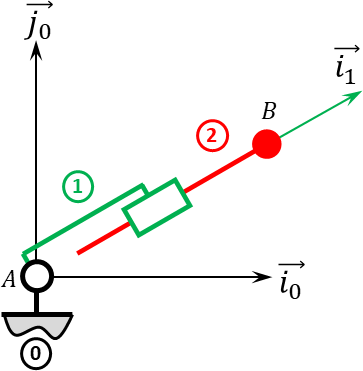
\includegraphics[width=.8\linewidth]{05_RT_01}
\end{center}
\fi


% ================================
\ifprof
\else
\ifcolle
\else
\marginnote{
\begin{solution}
\begin{enumerate}
\item $\vectv{B}{2}{0} =\dot{\lambda}(t)\vect{i_1}+\lambda(t)\dot{\theta}(t)\vect{j_1}$.
\item $\vectv{B}{2}{0}=\dot{\lambda}(t)\vi{1}+\lambda(t)\dot{\theta}(t)\vj{1}$.
\item $\torseurcin{V}{2}{0} =\torseurl{\dot{\theta}(t)\vk{0}}{\dot{\lambda}(t)\vi{1}+\lambda(t)\dot{\theta}(t)\vj{1}}{B}$.
\item $\vectg{B}{2}{0} =  \left( \ddot{\lambda}(t)-\lambda(t)\dot{\theta}(t)^2\right)\vi{1}  +  \left( \dot{\lambda}(t)\dot{\theta}(t) +\dot{\lambda}(t)\dot{\theta}(t)\right) \vj{1}$.
\end{enumerate}
\end{solution}}
\fi
\marginnote{Corrigé  voir \ref{B2:13:05:02}.}
\fi
% ================================



\question{Déterminer $\vectv{B}{2}{0}$ par dérivation vectorielle.}
\ifprof  ~\\
$\vectv{B}{2}{0} = \deriv{\vect{AB}}{\rep{0}}$ $=\deriv{\lambda(t)\vect{i_1}}{\rep{0}}$
$=\dot{\lambda}(t)\vect{i_1}+\lambda(t)\dot{\theta}(t)\vect{j_1}$.
\else
\fi


\question{Déterminer $\vectv{B}{2}{0}$ par composition.}
\ifprof ~\\
$\vectv{B}{2}{0}=\vectv{B}{2}{1}+\vectv{B}{1}{0}$.

$\forall P$, $\vectv{P}{2}{1}=\dot{\lambda}(t)\vi{1}$.

Par ailleurs $\babarv{B}{A}{1}{0}=-\lambda(t)\vi{1}\wedge\dot{\theta}(t)\vk{0}$
$=\lambda(t)\dot{\theta}(t)\vj{1}$.

Au final, $\vectv{B}{2}{0}=\dot{\lambda}(t)\vi{1}+\lambda(t)\dot{\theta}(t)\vj{1}$.

\else
\fi

\question{Donner le torseur cinématique $\torseurcin{V}{2}{0}$ au point $B$.}
\ifprof  ~\\
$\torseurcin{V}{2}{0} = \torseurl{\dot{\theta}(t)\vk{0}}{\dot{\lambda}(t)\vi{1}+\lambda(t)\dot{\theta}(t)\vj{1}}{B}$.
\else
\fi

\question{Déterminer $\vectg{B}{2}{0}$.}
\ifprof  ~\\
$\vectg{B}{2}{0} = \deriv{\vectv{B}{2}{0}}{\rep{0}}$
$ = \ddot{\lambda}(t)\vi{1}+  \dot{\lambda}(t)\dot{\theta}\vj{1}+\dot{\lambda}(t)\dot{\theta}\vj{1}-\lambda(t)\dot{\theta}(t)^2\vi{1}$
$ = \left( \ddot{\lambda}(t)-\lambda(t)\dot{\theta}(t)^2\right)\vi{1}  +  \left( \dot{\lambda}(t)\dot{\theta}(t) +\dot{\lambda}(t)\dot{\theta}(t)\right) \vj{1}$.
\else
\fi

